\section{Introducció i Funcionalitat}

El radio altímetre és un dispositiu electrònic essencial posicioant a bord d'una aeronau destinat a \textbf{proporcionar mesures acurades de l'altitud absoluta a la que es troba l'aeronau respecte el terreny}. 
Aquests, estàn dissenyats per a funcionar durant tota la vida útil de l'aeronau en la cual están instal·lats (uns 30 anys) i per tant per fer front un ampli rang d'operacions tenint en compte les possibles tolerancies produides per l'edat dels equips.

Els sistema de radio altímetre d'una aeronau esta format per tres tranceptors idèntics i l'equipament associat a cada un d'ells. Totes tres unitats operen de manera simultania i independent en la banda de 4.2 - 4.4 GHz (banda aeronautica destinada exclusivament per funcions de radionavegació) emetent un senyal i processant el senyal rebotat rebut en forma d'alçada.

Actualment, existeixen dos tipus d'altímetres que difereixen en el sistema de modulació del senyal emès: 
\begin{itemize}
\item Ona continua modelada en freqüència \textit{(FMCW)}
\item Modulació de pols \textit{(pulse modulation)}
\end{itemize}


\section{Aplicacions}

Els radio altímetres són uns components essencials per l'aeronavegació doncs proporcionen informació útil per l'execució de diverses operacions que garanteixen la seguretat de les aeronaus. Aquestes operacions són les següents:

\textbf{Sistemes automàtics de constrol de vol}

Els sistemes de control de vol de les aeronaus depenen de la informació d'alçada proporcionada pels radio altímetres a bord per tal de coneixer en tot moment la distància absoluta de les aeronaus respecte el terreny i així poder garantir la seguretat amb la seva correcte actuació.

\textbf{Aproximació i aterratge d'aeronaus}

Durant la fase d'aproximació d'una aeronau el radio altímetre, juntament amb altres sistemes mesuradors de distancia i sistemes d'aterratge, proporciona informació d'altitud respecte a terra de l'aeronau que els sistemes de control de vol d'abord utilitzen per ajustar l'aeronau als parametres establetrs d'aterratge. Arribats a certa alçada, al iniciar-se la fase d'aterratge els radio altímetres són els únics components proporcionant mesures d'alçada vertical que son utilitzades pel sistema d'autopilot per efectuar l'aterratge.  

Si el sistema de radio altímetres d'una aeronau no funciona o proporciona dades erronies les conseqüències van des de la necessitat de realitzar un aterratge manual en visual (sense autopilot) si l'aeroport ho permet i la visibilitat es bona a la necessitat de desviar-se a una aeroport proper que ho permeti o a esperar a una millora del temps. 

\textbf{Sistema d'alerta de proximitat al sól}

El sistema d'alerta de proximatat al sòl a bord de les aeronaus està dissenyat per evitar colisions així com evitar l'excesiu apropropament de l'aeronau a obstacles situats sota aquesta garantint la seva seguretat. Per fer-ho proporciona de manera automàtica avisos de proximitat de terrent sota l'aeronau a la tripulació.  

Els diferents tipus o modes d'avisos proporcionats per aquest sistema són el següents:
\begin{itemize}
\item Rati de descens elevat
\item Rati d'aproximació a terra excessiu
\item Pèrdua d'altitud durant enlairament
\item Espai no segur per proximitat a terra
\item Desviació excesiva respecta la \textit{senda de planeo}
\end{itemize}
Com es pot apreciar, tots aquest avisos están basats en l'altitud de l'aeronau respecte el sól a sota d'aquesta i per tant depenen de la informació proporcionada pels radio altímetres. 


\section{Models Comercials}

En aquesta secció és presenten diversos models comercials de radio altímetres juntament amb les seves especificacions.

\textbf{Radio Altimetre RA 4000$/$4500}

	\begin{figure}[H]
	\centering
	  \begin{subfigure}[b]{0.32\textwidth}
	  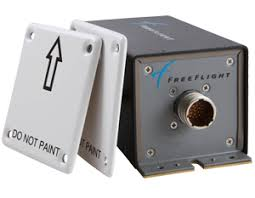
\includegraphics[width=\textwidth]{./images/RA4000.png}
	  \caption{}
	  \label{1diag1}
	  \end{subfigure}
	  \qquad %~ %add desired spacing between  images, e. g. ~, \quad,  \qquad, \hfill etc. 
	  \begin{subfigure}[b]{0.6\textwidth}
	  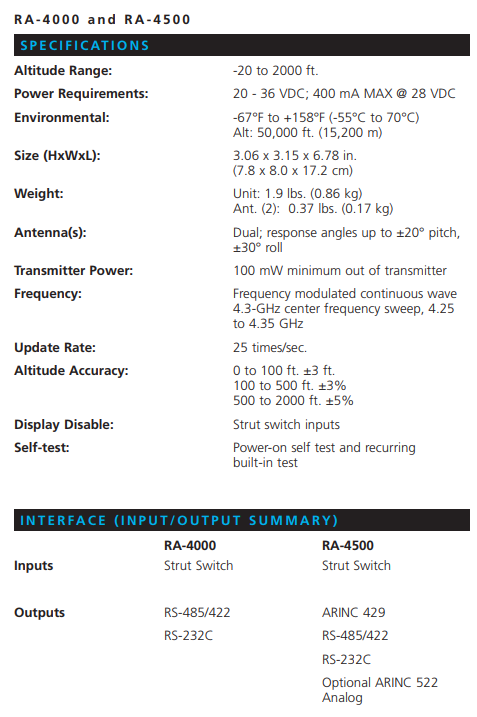
\includegraphics[width=\textwidth]{./images/RA4000Specs.png}
	  \caption{}
	  \label{1diag2}
	  \end{subfigure}
	  \vspace{10pt}
	\caption{}
	\label{diag1}
	\end{figure}






